% Chapter 5: Results and Discussion
This chapter presents the experimental results, comparing model performances across head, middle, and tail classes, and discussing the impact of different model architechtures combined with differnt loss functions. First, the main findings are presented, followed by a detailed analysis of the results across experiments, and lastly a discussion of the results. 

% \section{Overview}
% Present the performance of all tested models and methods.
% Use tables or plots to summarize key results.
% Highlight trends or notable observations across the methods.

\section{Main Findings}
% 1. Complete "Main Findings" Section
% This is the most critical part to finalize, as it sets the tone for the rest of the results chapter.
% Go through your tables and add specific examples of findings for each claim. For example:
% "Balanced Softmax consistently improved tail-class accuracy across all models, with a notable improvement in MobileNetV2 (Acc1: 0.9211)."
% "LDAM performed comparably on middle classes but struggled on head classes, as observed in ResNet50V2 (Acc1: 0.7983)."
% This will eliminate the TODO placeholders and give the reader a clear summary of the results.


Across all models, Balanced Softmax Loss demonstrated the highest performance on tail classes for models trained on long-tailed datasets while maintaining consistent performance on head, middle, and overall long-tailed test sets. The highest top-1 accuracy for tail classes was achieved by the ResNet50V2 architecture (Acc1: 0.6053), closely followed by the ConvNeXt Base architecture (Acc1: 0.5789). However, this improved tail-class performance comes at the cost of head-class accuracy, where ConvNeXt Base outperforms ResNet50V2 with a top-1 accuracy of 0.8685 compared to 0.8270. Overall, ConvNeXt Base demonstrates better performance across all classes (Acc1: 0.8230) compared to ResNet50V2 (Acc1: 0.7916). See Tables \ref{tab:resnet_lt_acc1_1} and \ref{tab:conv_lt_acc1_1} for reference. These results, however, require further statistical analysis to establish their significance.



Class-Balanced Loss consistently underperformed, warranting further investigation into its implementation. Similarly, the ViT-B/16 architecture demonstrated the lowest overall accuracy when trained on both balanced and long-tailed datasets (Acc1: 59.06 \%, see Table \ref{tab:vit_bal_acc1_1}), despite having the highest reported benchmark performance (Acc1: 93.95 \%) among all model architectures investigated in this thesis \cite{Tseng_2022}. This discrepancy suggests potential limitations in its design or configuration.


\section{Overall Results}
This section presents the overall results of all experiments conducted in this thesis, commenting on the best and worst performance of loss designs on a given model, and not directly comparing loss designs or models. This section is meant as an overview of all findings.

\subsection{MobileNetV2}

\subsubsection{Results from Balanced Training Dataset}

\begin{table}[H]
    \centering
    \caption{Top-1 accuracy results for MobileNetV2 on the balanced dataset across all loss functions.}
    \begin{tabular}{cccccc}
        \toprule
        Loss Function & Balanced & Long-tailed & Head & Middle & Tail \\ 
        \midrule
        Softmax   & 0.7978   & \textbf{0.8059} & \textbf{0.8069} & \textbf{0.7870} & 0.8684 \\
        Focal loss   & 0.8014   & 0.8011 & 0.7998 & \textbf{0.7870} & 0.8947 \\
        Weighted Softmax loss   & 0.7978   & \textbf{0.8059} & \textbf{0.8069} & \textbf{0.7870} & 0.8684 \\
        Class-balanced loss   & 0.7978   & \textbf{0.8059} & \textbf{0.8069} & \textbf{0.7870} & 0.8684 \\
        Balanced Softmax loss   & \textbf{0.8034}  & 0.8030 & \textbf{0.8069} & 0.7574 & \textbf{0.9211} \\
        Equalization loss   & 0.7994   & 0.8040 & 0.8057 & 0.7692 & \textbf{0.9211} \\
        LDAM loss   &  0.7828   & 0.7821 & 0.7808 & 0.7574 & \textbf{0.9211} \\
        \bottomrule
    \end{tabular}
    \label{tab:mobilenet_bal_acc1_1}
\end{table}

\begin{figure}[h!]
    \centering
    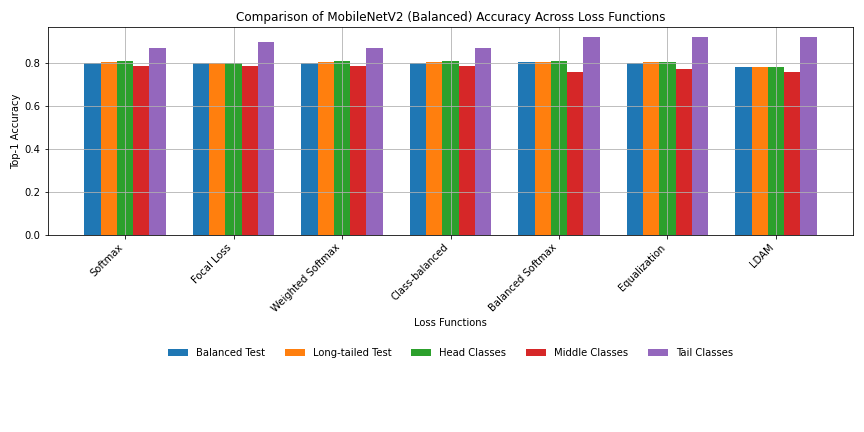
\includegraphics[width=\textwidth]{Images/Plots/mobilenet_bal_loss_comparison.png}
    \caption{Top-1 accuracy comparison of MobileNetV2 trained on the balanced CIFAR-100 across loss functions on different test datasets. The bars represent performance on balanced test data, long-tailed test data, and head, middle, and tail classes.}
    \label{fig:mobilenet_bal_loss_comparison}
\end{figure}

\todo{Comment on \ref{fig:mobilenet_bal_loss_comparison}.}

From Table \ref{tab:mobilenet_bal_acc1_1}, the overall best performance on MobileNetV2 trained with a balanced CIFAR100 training dataset is achieved by Balanced Softmax Loss, which has the highest accuracy on the balanced test dataset (Acc1: 0.8034), as well as on the head (Acc1: 0.8069) and tail (Acc1: 0.9211) classes, with only slightly worse performance on the middle classes in comparison. Among all loss functions, LDAM Loss shows the lowest overall performance on the balanced test set (Acc1: 0.7828) and the long-tailed test set (Acc1: 0.7821), except for its strong performance on tail classes (Acc1: 0.9211). % This highlights LDAM’s specialized focus on tail classes at the cost of performance on head and middle classes.

Softmax Loss, Weighted Softmax Loss, and Class-Balanced Loss yield the same accuracies across all test datasets, likely due to their similarities in loss design  \todo{Refer to background section}.

Balanced Softmax Loss, Equalization Loss, and LDAM Loss exhibit the highest accuracy on tail classes (Acc1: 0.9211). Despite their differing loss designs, this convergence in accuracy suggests that the dataset's tail-class performance may have reached a plateau, possibly due to the inherent characteristics of the tail classes, i.e. either noise or the limited number of samples available per class in the tail \todo{Refer to background section}.

A similar trend is observed in the middle-class accuracy, where Softmax, Focal Loss, Weighted Softmax Loss, and Class-Balanced Loss all achieve identical results (Acc1: 0.7870). Similarly, for head classes, Softmax, Weighted Softmax Loss, Class-Balanced Loss, and Balanced Softmax Loss perform equally well, achieving the highest accuracy (Acc1: 0.8069). % hinting at saturation. This consistency across different loss functions on the balanced dataset could be due to their shared design principles.

% TODO: Compare results to related studies of MobileNetV2 trained on CIFAR100 [table \ref{tab:comparison_mobilenet}]. Mention that the results from MobileNetV2 on the balanced CIFAR100 are okay but not the greatest.




% However, because balanced softmax loss does not yield the same result on both the balanced test set and the long-tailed test set as the other three mentioned, it is likely due to a saturation in the head classes. The softmax loss, weighted softmax loss, and class-balanced loss all yield the same performance across test sets, showing their similiarity in loss design on a balanced training dataset. The best perfoming loss function on the balanced test set is the weighted softmax loss (Acc1: 0.8034), however this is not the best performing loss function on the complete long-tailed dataset, but it has the best accuracy on tail classes (Acc1: 0.9211), and comparable performance on head and tail classes. Except for the performance on tail classes, the overall worst performing loss method is the LDAM loss, with accuracy of 0.7828 on a balanced test set, and 0.7821 on a long-tailed test set. Compared to the baseline, the softmax loss, that has an accuracy of 0.7978 on the balanced test set, and 0.8059 on the long-tailed test set.


% Balanced Softmax Loss, however, stands out due to its differentiated performance across datasets. Unlike Softmax, Weighted Softmax Loss, and Class-Balanced Loss, which yield consistent results across balanced and long-tailed datasets, Balanced Softmax achieves a higher accuracy on tail classes while showing slight variability in overall performance. This suggests that Balanced Softmax is more sensitive to class-specific adjustments, particularly in imbalanced scenarios.


% 
% Compared to the baseline Softmax Loss (balanced: Acc1: 0.7978, long-tailed: Acc1: 0.8059), Balanced Softmax Loss demonstrates slightly better performance on the balanced dataset but shows more variability on the long-tailed dataset, where it achieves comparable results on tail classes but lower performance overall.

\subsubsection{Results from Long-Tailed Training Dataset}

Table \ref{tab:mobilenet_lt_acc1_1} shows the top 1 accuracies for MobileNetV2 on all loss functions.

\begin{table}[H]
    \centering
    \caption{Top-1 accuracy results for MobileNetV2 on the long-tailed dataset across all loss functions.}
    \begin{tabular}{cccccc}
        \toprule
        Loss Function & Balanced & Long-tailed & Head & Middle & Tail \\ 
        \midrule
        Softmax   & 0.5282   & 0.7735 & 0.8341 & 0.5917 & 0.2368 \\
        Focal loss   & 0.5200   & \textbf{0.7745} & \textbf{0.8389} & 0.5917 & 0.1579 \\
        Weighted Softmax loss   & 0.5016   & 0.7231 & 0.7808 & 0.5503 & 0.2105 \\
        Class-balanced loss   & 0.1936   & 0.0913 & 0.0521 & 0.2485 & 0.2632 \\
        Balanced Softmax loss   & \textbf{0.5796}   & 0.7650 & 0.8069 & \textbf{0.6331} & \textbf{0.4211} \\
        Equalization loss   & 0.5310   & 0.7650 & 0.8235 & 0.5917 & 0.2368 \\
        LDAM loss   & 0.4264 & 0.5899 & 0.6137 & 0.5444 & 0.2632 \\
        \bottomrule
    \end{tabular}
    \label{tab:mobilenet_lt_acc1_1}
\end{table}

\begin{figure}[h!]
    \centering
    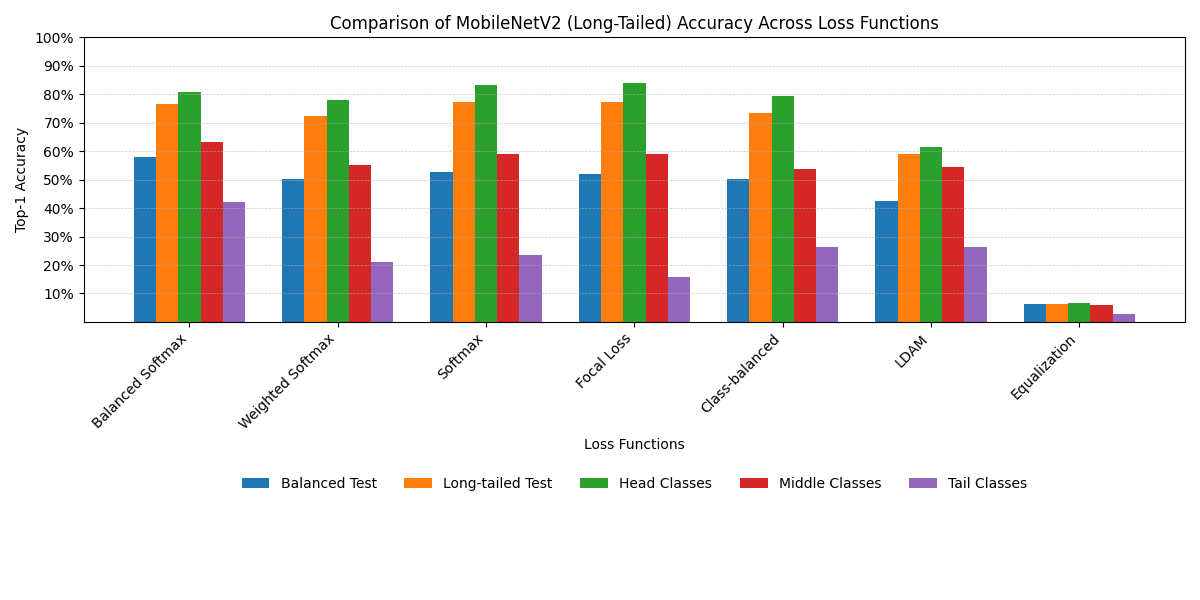
\includegraphics[width=\textwidth]{Images/Plots/mobilenet_lt_loss_comparison.png}
    \caption{Top-1 accuracy comparison of MobileNetV2 trained on the long-tailed CIFAR-100 across loss functions on different test datasets. The bars represent performance on balanced test data, long-tailed test data, and head, middle, and tail classes.}
    \label{fig:mobilenet_lt_loss_comparison}
\end{figure}

\todo{Comment on figure \ref{fig:mobilenet_lt_loss_comparison}.}

From table \ref{tab:mobilenet_lt_acc1_1}, the best overall performance on MobileNetV2 trained with a long-tailed CIFAR100 training dataset is achieved by Balanced Softmax Loss, with the highest accuracy on the balanced test set (Acc1: 0.5796), middle classes (Acc1: 0.6331), and tail classes (Acc1: 0.4211), and with competing accuracies on the long-tailed test dataset (Acc1: 0.7650) and head classes (Acc1: 0.8069), with the highest performance of Focal Loss with top-1 accuracies of 0.7745 and 0.8389, respectively.

The Class-Balanced loss exhibits the least satisfactory accuracies across all test dataset (Balanced: 0.1936, Long-Tailed: 0.0913, Head: 0.0521, Middle: 0.2485), with the only exception at tail classes (Acc1: 0.2632), where the results are comparable to those of other loss designs. This is a contrast to the performance when trained with a balanced CIFAR100 dataset, where the loss design performed within range of the other loss designs, possibly indicating a fault in implementation \todo{investigate implementation}.

Unlike the performance of loss functions trained on the balanced CIFAR100, there are not as many incidents of accuracies of the same value, except for the performance of Softmax Loss, Focal Loss, and Equalization loss on middle classes (Acc1: 0.5917). However, this value is not the highest, as the Balanced Softmax Loss achieves a top-1 accuracy of 0.6331. \todo{explain this.}

\subsubsection{Comparison to Benchmark}
\todo{No benchmark for MobileNetV2 trained on CIFAR-100.}
The paper \textit{BiTAT: Neural Network Binarization
with Task-dependent Aggregated Transformation} by Park et al. tested a MobileNetV2 architecture on CIFAR100 with the highest top 1 accuracy of 73.20 \% .
Link to paper: \url{https://arxiv.org/pdf/2207.01394}

The paper \textit{E$^2$-Train: Training State-of-the-art CNNs with Over
80\% Energy Savings} by Wang et al. reported a top 1 accuracy of 71.91 \% with MobileNetV2 evaluated on CIFAR100.
Link to paper: \url{https://arxiv.org/pdf/1910.13349}

Mine is 80.34 \%. See table \ref{tab:mobilenet_bal_acc1_1}.
% The comparison of my experiment to the original MobileNetV2 trained on the original CIFAR100 dataset.

% Table \ref{tab:comparison_mobilenet} compares the experimental setup and results of MobileNetV2 trained on the CIFAR100 dataset with those reported in Study A3. Key differences include the loss function, optimizer, and data augmentation techniques used.

% While our approach achieves competitive top-1 accuracy on balanced datasets, the performance gap on long-tailed datasets highlights potential areas for improvement in augmentation and learning rate strategies.

% TODO: Move comparisons of results to a seperate section. Keep only the results, put specification in an appendix.

% \begin{table}[H]
%     \centering
%     \begin{tabular}{lp{5cm}p{5cm}}
%         \toprule
%         \textbf{Aspect} & \textbf{Your Experiment} & \textbf{Their Study (A3)} \\ 
%         \midrule
%         Dataset            & CIFAR100 Customized                & CIFAR100                \\
%         Loss Function      & Softmax Cross-Entropy   & Binary Cross-Entropy    \\
%         Epochs             & 90                      & 100                     \\
%         Optimizer          & Adam                    & LAMB                    \\
%         Learning Rate      & Step decay at 30, 60 epochs & Cosine decay from 0.005 or 0.008 \\
%         Augmentation       & Resize (224x224), RandomCrop, Horizontal Flip, Normalize & RandAugment, Mixup, CutMix, Normalize \\
%         Hardware           & 4x NVIDIA TITAN X (Pascal, 12GB) & 4x NVIDIA V100 (32GB) \\
%         Evaluation Metric  & Top-1 Accuracy          & Top-1 Accuracy          \\
%         Top-1 Accuracy     & 79.8 \% & 86.2\%-86.9\%           \\
%         \bottomrule
%     \end{tabular}
%     \caption{Comparison of MobileNetV2 on CIFAR100 with their study (Procedure A3) \cite{wightman2021resnetstrikesbackimproved}.}
%     \label{tab:comparison_mobilenet}
% \end{table}


\subsection{ResNet50V2}

\subsubsection{Results from Balanced Training Dataset}

Table \ref{tab:resnet_bal_acc1_1} show the top 1 accuracies for ResNet50V2 on all loss functions.

\begin{table}[H]
    \centering
    \caption{Evaluation results for ResNet50V2 trained on the custom balanced dataset, showing Acc1.}
    \begin{tabular}{cccccc}
        \toprule
        Loss Function & Balanced & Long-tailed & Head & Middle & Tail \\ 
        \midrule
        Softmax loss   & \textbf{0.8324}  & 0.8421 & 0.8448 & 0.8047 & \textbf{0.9474} \\
        Focal loss   & 0.8310  & 0.8344 & 0.8341 & \textbf{0.8166} & 0.9211 \\
        Weighted Softmax loss   & \textbf{0.8324} & 0.8421 & 0.8448 & 0.8047 & \textbf{0.9474} \\
        Class-balanced loss   &  \textbf{0.8324} & 0.8421 & 0.8448 & 0.8047 & \textbf{0.9474} \\
        Balanced Softmax loss   & 0.8310 & \textbf{0.8430} & \textbf{0.8460} & 0.8107 & 0.9211 \\
        Equalization loss   & 0.8292 & 0.8373 & 0.8412 & 0.7929 & \textbf{0.9474} \\
        LDAM loss   & 0.7990 & 0.7983 & 0.8069 & 0.7337 & 0.8947 \\
        \bottomrule
    \end{tabular}
    \label{tab:resnet_bal_acc1_1}
\end{table}

From table \ref{tab:resnet_bal_acc1_1}, there are three loss designs with the best perfomance on the balanced test dataset, namely Softmax Loss, Weighted Softmax Loss, and Class-Balanced Loss (Acc1: 0.8324). Furthermore, they all yeild the same results across all test dataset due to their cross-entropy architecture for balanced training data. Likewise they yield the best perfomance on the tail classes along with equalization loss (Acc1: 0.9474) \todo{explain}. % possibly due to the low number of samples in the tail classes.

The perfomance of the Balanced Softmax Loss shows excellence on the long-tailed dataset (Acc1: 0.8430) as well as the head classes (Acc1: 0.8460) with competing results on both middle (Acc1: 0.8107) and tail (Acc1: 0.9211) classes.

The worst performance is that of the LDAM loss across all test datasets.

\subsubsection{Results from Long-Tailed Training Dataset}

Table \ref{tab:resnet_lt_acc1_1} show the top 1 accuracies for ResNet50V2 on various loss functions.

\begin{table}[H]
    \centering
    \caption{Evaluation results for ResNet50V2 trained on the long-tailed dataset, showing Acc1.}
    \begin{tabular}{cccccc}
        \toprule
        Loss Function & Balanced & Long-tailed & Head & Middle & Tail \\ 
        \midrule
        Softmax loss   & 0.5522 & \textbf{0.7954} & \textbf{0.8531} & 0.6391 & 0.2105 \\
        Focal loss   & 0.5456 & 0.7935 & 0.8483 & 0.6272 & 0.3158 \\
        Weighted Softmax loss   & 0.4976 & 0.7336 & 0.7915 & 0.5562 & 0.2368 \\
        Class-balanced loss   & 0.2052 & 0.1836 &  0.1445 & 0.3787 & 0.1842 \\
        Balanced Softmax loss   & \textbf{0.5908} & 0.7916 & 0.8270 & \textbf{0.6568} & \textbf{0.6053} \\
        Equalization loss   & 0.5452 & 0.7897 & 0.8389 & 0.6450 & 0.3421 \\
        LDAM loss   & 0.3742 & 0.5937 & 0.6469 & 0.4438 & 0.0789 \\
        \bottomrule
    \end{tabular}
    \label{tab:resnet_lt_acc1_1}
\end{table}


From table \ref{tab:resnet_lt_acc1_1}, the performance of the Balanced Softmax Loss present the best on the balanced dataset (Acc1: 0.5906), middle (Acc1: 0.6568), and tail classes (Acc1: 0.6053) with competing perfomances on the long-tailed datsaet (Acc1: 0.7916) and head classes (Acc1: 0.8270). The best performance on the long-tailed dataset and head classes was presented by the Softmax Loss (Acc1: 0.7954, 0.8531).

Two loss designs are competing for the worst performance with underwhelming results across all test datasets, namely the Class-Balanced loss and the LDAM loss. The LDAM loss achieved an accuracy of 0.0789 on the tail classes, while remaining stable, but unsatisfactory on the rest. The Class-balanced loss with the highest accuracy of 0.3787 across all test datasets has a performance of negligence.

\subsubsection{Comparison to Benchmark}
\todo{No benchmark for ResNet50V2 trained on CIFAR-100. Closest architecture is ResNet50 from the paper \textit{ResNet strikes back: An improved training procedure in timm} \cite{wightman2021resnetstrikesbackimproved}.}

Top 1 accuracy trained on a balanced CIFAR100:
Their: 86.9 \%.
Mine: 83.2 \%.

\todo{Describe differences.}

\subsection{ViT-B/16}

\subsubsection{Results from Balanced Training Dataset}

\begin{table}[H]
    \centering
    \caption{Evaluation results for ViT-B/16 trained on the custom balanced dataset, showing Acc1.}
    \begin{tabular}{cccccc}
        \toprule
        Loss Function & Balanced & Long-tailed & Head & Middle & Tail \\ 
        \midrule
        Softmax loss   & 0.5620 & 0.5671 & 0.5521 & 0.6036 & 0.7368 \\
        Focal loss   & 0.5516 & 0.5538 & 0.5438 & 0.5680 & 0.7105 \\
        Weighted Softmax loss   & 0.5620 & 0.5671 & 0.5521 & 0.6036 & 0.7368 \\
        Class-balanced loss   & 0.5620 & 0.5671 &  0.5521 & 0.6036 & 0.7368 \\
        Balanced Softmax loss   & 0.5628 & 0.5642 & 0.5640 & 0.5325 & 0.7105 \\
        Equalization loss   & 0.5634   & 0.5519 & 0.5462 & 0.5503 & 0.6842 \\
        LDAM loss   & \textbf{0.5906} &  \textbf{0.6013} & \textbf{0.5924} & \textbf{0.6095} & \textbf{0.7632} \\
        \bottomrule
    \end{tabular}
    \label{tab:vit_bal_acc1_1}
\end{table}

From table \ref{tab:vit_bal_acc1_1} it is clear that the loss design with the overall best perfomance on the ViT-B/16 architechture is the LDAM loss. However, the performance of all loss designs across all test datasets are noticably worse than the performance of the other model architectures in this experiment trained with the balanced training dataset. See tables \ref{tab:mobilenet_bal_acc1_1}, \ref{tab:resnet_bal_acc1_1}, and \ref{tab:conv_bal_acc1_1} for reference.  

There is no noticably trend in overall worst performance across loss designs, as all loss function perform within range of each other on all datasets.

\todo{Consider if it make sense to calculate the standard deviation of results within datasets.}  

\subsubsection{Results from Long-Tailed Training Dataset}

\begin{table}[h!]
    \centering
    \caption{Evaluation results for ViT-B/16 trained on the long-tailed dataset, showing Acc1.}
    \begin{tabular}{cccccc}
        \toprule
        Loss Function & Balanced & Long-tailed & Head & Middle & Tail \\ 
        \midrule
        Softmax loss   & 0.2254 & \textbf{0.4367} & \textbf{0.5071} & 0.1775 & 0.0263 \\
        Focal loss   & 0.2210 & 0.4206 & 0.4834 & 0.1953 & 0.0263 \\
        Weighted Softmax loss   & 0.1284 & 0.1760 & 0.1919 & 0.1302 & 0.0263 \\
        Class-balanced loss   & 0.0558 & 0.0076 & 0.0000 & 0.0237 & \textbf{0.1053} \\
        Balanced Softmax loss   & \textbf{0.2460} & 0.4244 & 0.4822 &  \textbf{0.2130} & 0.0789 \\
        Equalization loss   & 0.2168 & 0.4215 & 0.4893 & 0.1716 & 0.0263 \\
        LDAM loss   & 0.1570 & 0.2750 & 0.3140 & 0.1361 & 0.0263 \\
        \bottomrule
    \end{tabular}
    \label{tab:vit_lt_acc1}
\end{table}

From table \ref{tab:vit_lt_acc1}, the best perfomance on the balanced test dataset is accomplshed by th Balanced Softmax loss (Acc1: 0.2460) which also has the best perfomance on middle classes (Acc1: 0.2130), while the Softmax loss achieves the best performance on the long tailed dataset (Acc1: 0.4367) as well as the head classes (0.5071). The best performance on tail classes is achieved by the Class-Balanced loss (Acc1: 0.1053) \todo{check this again}, however this loss design has an underwhelming performance across all other test sets with the lowest achieved perfomance on the head classes with 0.000 accuracy \todo{explain}. 

In all tests, the only loss design achieving a higher accuracy than 50 \% is the Softmax loss on the head classes, meaning that the model underperforms across all loss designs.

\subsubsection{Comparison to Benchmark}
The best result from ViT-B/16 trained with CIFAR100 is obtained in \textit{Perturbated Gradients Updating within Unit Space for Deep Learning} \cite{Tseng_2022} with the best accuracy of 93.95 \%. In comparison, the highest achieved accuracy on a balanced test dataset in this experiment on ViT-B/16 trained with a balanced CIFAR100 was 59.1 \%. See table \ref{tab:vit_bal_acc1_1}. \todo{Compare methods.}
Link to paper: \url{https://arxiv.org/pdf/2110.00199v2}

\todo{Make a table with results.}

% \todo{Move comparisons of results to a seperate section. Keep only the results, put specification in an appendix.}

% \begin{table}[h!]
%     \centering
%     \renewcommand{\arraystretch}{1.2} % Adjust row spacing
%     \setlength{\tabcolsep}{4pt} % Adjust column spacing
%     \begin{tabular}{lp{6cm}p{6cm}}
%         \toprule
%         \textbf{Aspect} & \textbf{Your Experiment} & \textbf{PUGD Results} \\ 
%         \midrule
%         Dataset           & CIFAR100 & CIFAR100 \\
%         Model             & ViT-B/16 pretrained on ImageNet-21K & Multiple models: VGG-16, ResNet-18, DenseNet-121, UPANet-16, and ViT-B/16 \\
%         Pretraining       & ImageNet-21K & ImageNet-1K (for fine-tuned models) \\
%         Optimizer         & Adam & PUGD \\
%         Loss Function     & Softmax Cross-Entropy & Softmax Cross-Entropy \\
%         Epochs            & 90 & 200 (end-to-end); 80–100 (fine-tuning) \\
%         Learning Rate     & Step decay: 0.001 → 0.0001 → 0.00001 & Cosine Annealing: 0.1 (end-to-end); 0.01–0.005 (fine-tuning) \\
%         Augmentation      & Resize (224), RandomCrop, Horizontal Flip, Normalize & Resize (224), RandAugment, Cutout, Normalize \\
%         Top-1 Accuracy    & - & End-to-End: Up to 78.30\% (DenseNet-121); Fine-tuning: ViT-B/16 achieves 93.95\% \\
%         Hardware          & 4x NVIDIA TITAN X (Pascal, 12GB) & RTX-Titan, 32GB RAM, eight-core processor \\
%         \bottomrule
%     \end{tabular}
%     \caption{Comparison of my experiment with PUGD results on CIFAR-100.}
%     \label{tab:comparison3}
% \end{table}


\subsection{ConvNeXt Base}

\subsubsection{Results from balanced Training Dataset}

\begin{table}[h!]
    \centering
    \caption{Evaluation results for ConvNeXt Base trained on the custom balanced dataset, showing Acc1.}
    \begin{tabular}{cccccc}
        \toprule
        Loss Function & Balanced & Long-tailed & Head & Middle & Tail \\ 
        \midrule
        Softmax loss   & 0.8332 & \textbf{0.8535} & \textbf{0.8566} & 0.8166 & \textbf{0.9474} \\
        Focal loss   & 0.8314 & 0.8487 & 0.8507 & 0.8284 & 0.8947 \\
        Weighted Softmax loss   & 0.8332 & \textbf{0.8535} & \textbf{0.8566} &  0.8166 & \textbf{0.9474} \\
        Class-balanced loss   & 0.8332 & \textbf{0.8535} & \textbf{0.8566} & 0.8166 & \textbf{0.9474} \\
        Balanced Softmax loss   & \textbf{0.8364} & 0.8344 & 0.8365 & 0.7988 & \textbf{0.9474} \\
        Equalization loss   & 0.8318 & 0.8468 & 0.8448 & \textbf{0.8343} & \textbf{0.9474} \\
        LDAM loss   & 0.8316 & 0.8373 & 0.8412 & 0.8047 & 0.8947 \\
        \bottomrule
    \end{tabular}
    \label{tab:conv_bal_acc1_1}
\end{table}

From table \ref{tab:conv_bal_acc1_1}, the best performance on the balanced test dataset is achieved by the Balanced Softmax Loss (Acc1: 0.8364), while also achieving the best result on the tail classes (Acc1: 0.9474).

Not surprisingly, the Softmax loss, Weighted Softmax loss, and Class-balanced loss exhibits the same performance across all test dataset, as they were trained with the balanced training dataset, and their designs reduces to the Softmax loss. These three loss function exhibit the best performance on the long-tailed dataset (0.8535), head classes (Acc1: 0.8566) and tail classes (Acc1: 0.9474). The best performance on middle classes is achieved my the Equalization loss (Acc1: 0.8343).

Five out of six loss design achieve the same performance on the tail classes, likely due to saturation causes by the limited number of samples and noise.

\todo{Explain why balanced softmax could achieve higher accuracy in the balanced dataset.}

\subsubsection{Results from Long-Tailed Training Dataset}


\begin{table}[h!]
    \centering
    \caption{Evaluation results for ConvNeXt Basetrained on the long-tailed dataset, showing Acc1.}
    \begin{tabular}{cccccc}
        \toprule
        Loss Function & Balanced & Long-tailed & Head & Middle & Tail \\ 
        \midrule
        Softmax loss   & 0.5972 & \textbf{0.8316} & \textbf{0.8898} & 0.6568 & 0.3158 \\
        Focal loss   & 0.5938 & 0.8145 & 0.8685 & 0.6568 & 0.3158 \\
        Weighted Softmax loss   & 0.4090 & 0.6356 & 0.6848 & 0.4911 & 0.1842 \\
        Class-balanced loss   & 0.0142 & 0.0019 & 0.0000 & 0.0000 & 0.0526 \\
        Balanced Softmax loss   & \textbf{0.6460} & 0.8230 & 0.8685 & 0.6509 & \textbf{0.5789} \\
        Equalization loss   & 0.5956 & 0.8278 & 0.8768 & \textbf{0.6923} & 0.3421 \\
        LDAM loss   & 0.3770 & 0.5956 & 0.6445 & 0.4260 & 0.2632 \\
        \bottomrule
    \end{tabular}
    \label{tab:conv_lt_acc1_1}
\end{table}

From table \ref{tab:conv_lt_acc1_1} the best performance on a balanced test dataset is achived by the Balanced Softmax loss (Acc1: 0.6460), which was the same for the ConvNeXt Base trained with the balanced CIFAR100. See table \ref{tab:conv_bal_acc1_1}. Likewise, the Balanced Softmax loss performs with the highest accuracy on the tail classes (Acc1: 0.5789), far exceeding the second highest performance, achieved by Equalization loss (Acc1: 0.3421). The highest accuracy on the long-tailed dataset (Acc1: 0.8316), as well as the head classes (Acc1: 0.8898), is achieved by the Softmax Loss, while Equalization Loss performs with highest accuracy on middle classes (Acc1: 0.6923). In comparison, the Balanced Softmax loss is third in accuracy on the long-tailed dataset, head classes, as well as middle classes. 

Noticably, both Softmax loss and focal loss performs with equal accuracies on both middle (Acc1: 0.6568) and tail classes (Acc1: 0.3158), but not elsewhere. \todo{give a reason why that might be.}

The worst performance is achieved by the Class-Balanced loss, with accuracies far below the second worst performances. The Class-balanced loss should be disregarded for training with a long-tailed dataset, as it is most likely a fault in implementation. \todo{investigate this and return to this conclusion.}


\subsubsection{Comparison to Benchmark}
\todo{No benchmark found for ConvNeXt Base trained with CIFAR100.}
Closest is \textit{Conv2NeXt: Reconsidering Conv NeXt Network Design for Image Recognition} by Feng et al. with top 1 accuracy of 83.82 \% in CIFAR-100. Mine is 83.64 \%.
Link: \url{https://ieeexplore.ieee.org/document/10072172}

\section{Comparison of Models}

The model are compared by taking the mean of the results of the loss functions for each model. The mean and standard deviation for each model are shown on figure \ref{fig:mean_loss_comparison_line}, and on figure \ref{fig:mean_loss_comparison_line_noCB} excluding the Class-Balanced Loss.

\begin{figure}[h!]
    \centering
    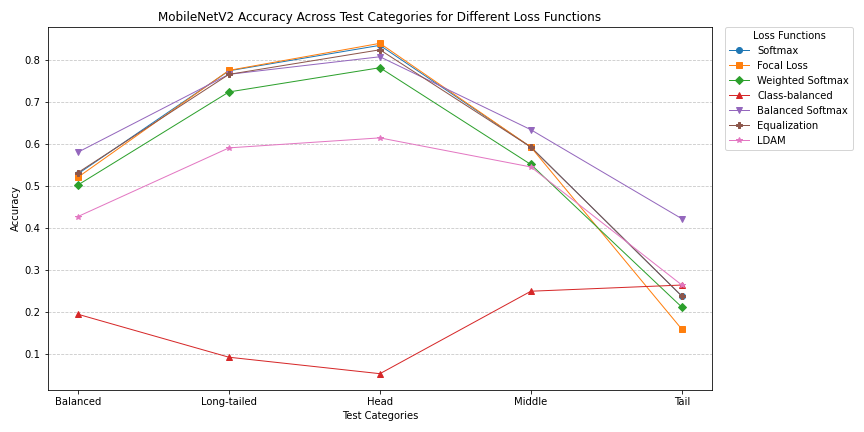
\includegraphics[width=\textwidth]{Images/Plots/mobilenet_lt_loss_comparison_line.png}
    \caption{MobileNetV2 top 1 accuracy across test categories (Balanced, Long-tailed, Head, Middle, Tail) for different loss functions.}
    \label{fig:mobilenet_bal_loss_comparison_line}
\end{figure}

\begin{figure}[h!]
    \centering
    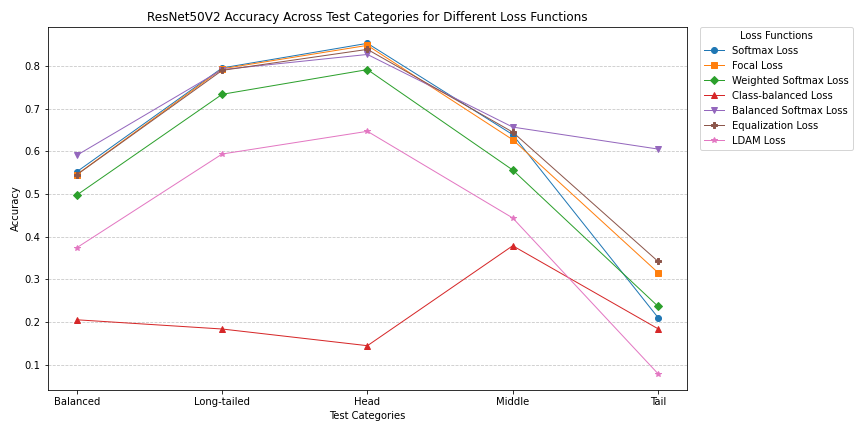
\includegraphics[width=\textwidth]{Images/Plots/resnet_lt_loss_comparison_line.png}
    \caption{ResNet50V2 top 1 accuracy across test categories (Balanced, Long-tailed, Head, Middle, Tail) for different loss functions.}
    \label{fig:resnet_bal_loss_comparison_line}
\end{figure}

\begin{figure}[h!]
    \centering
    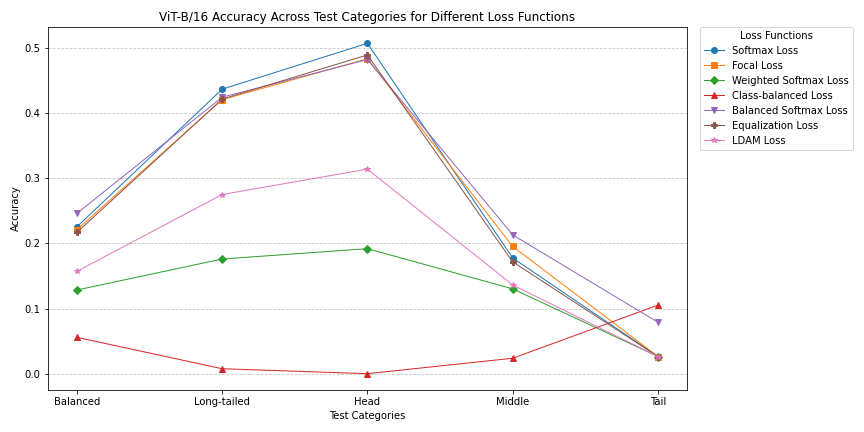
\includegraphics[width=\textwidth]{Images/Plots/vit_lt_loss_comparison_line.png}
    \caption{ViT-B/16 top 1 accuracy across test categories (Balanced, Long-tailed, Head, Middle, Tail) for different loss functions.}
    \label{fig:vit_bal_loss_comparison_line}
\end{figure}

\begin{figure}[h!]
    \centering
    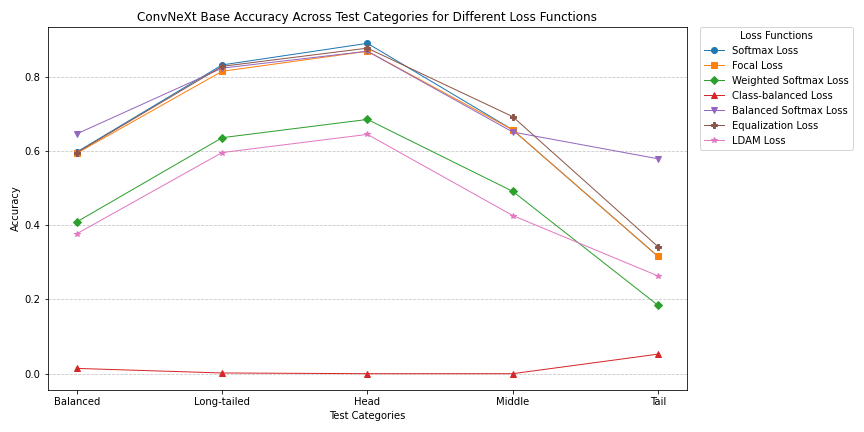
\includegraphics[width=\textwidth]{Images/Plots/convnext_lt_loss_comparison_line.png}
    \caption{ConvNeXt Base top 1 accuracy across test categories (Balanced, Long-tailed, Head, Middle, Tail) for different loss functions.}
    \label{fig:conv_bal_loss_comparison_line}
\end{figure}

\subsubsection{Mean and Standard Deviation}

\todo{Make a table for the mean and standard deviations.}

The plots on figures \ref{fig:mean_loss_comparison_line} and \ref{fig:mean_loss_comparison_line_noCB} compares the performance of the models MobileNetV2, ResNet50V2, ViT-B/16, and ConvNeXt Base across the evaluation categories: balanced, long-tailed, head, middle, and tail. Each model is slightly offset along the x-axis to avoid overlap. The mean and standard deviation in figure \ref{fig:mean_loss_comparison_line} include the Class-Balanced Loss while figure \ref{fig:mean_loss_comparison_line_noCB} does not.

Each point represents the mean accuracy of a model for a specific category and the bars represent the standard deviation. A model with higher mean accuracy is performing better in that category, and a smoother or higher line indicates consistent performance across all categories.

The error bars show the variability in accuracy across different loss functions for each model and category. A longer error bar means the performance is less consistent and the performance is more dependent on the chosen loss function, while shorter error bars indicate consistant performance.

The plot in figure \ref{fig:mean_loss_comparison_line_noCB} shows that the model with the best average performance on tail classes is the ConvNeXt Base architecture, while also showing a strong performance in other categories. 

MobileNetV2 is the least dependent on loss functions, exhibiting the smallest standard deviation, while the ResNet50V2 architecture, compared with figures \ref{fig:resnet_bal_loss_comparison_line} and \ref{fig:conv_bal_loss_comparison_line}, is the most dependent on loss functions when exhibiting tail performance, as the Balanced Softmax Loss outperforms the remaining loss functions, as seen in figure \ref{fig:resnet_bal_loss_comparison_line} and table \ref{tab:resnet_lt_acc1_1}.

The model exhibiting the worst performance is the ViT-B/16 with a significant lower mean than the other three models. \todo{reference to figures and tables.}

\begin{figure}[h!]
    \centering
    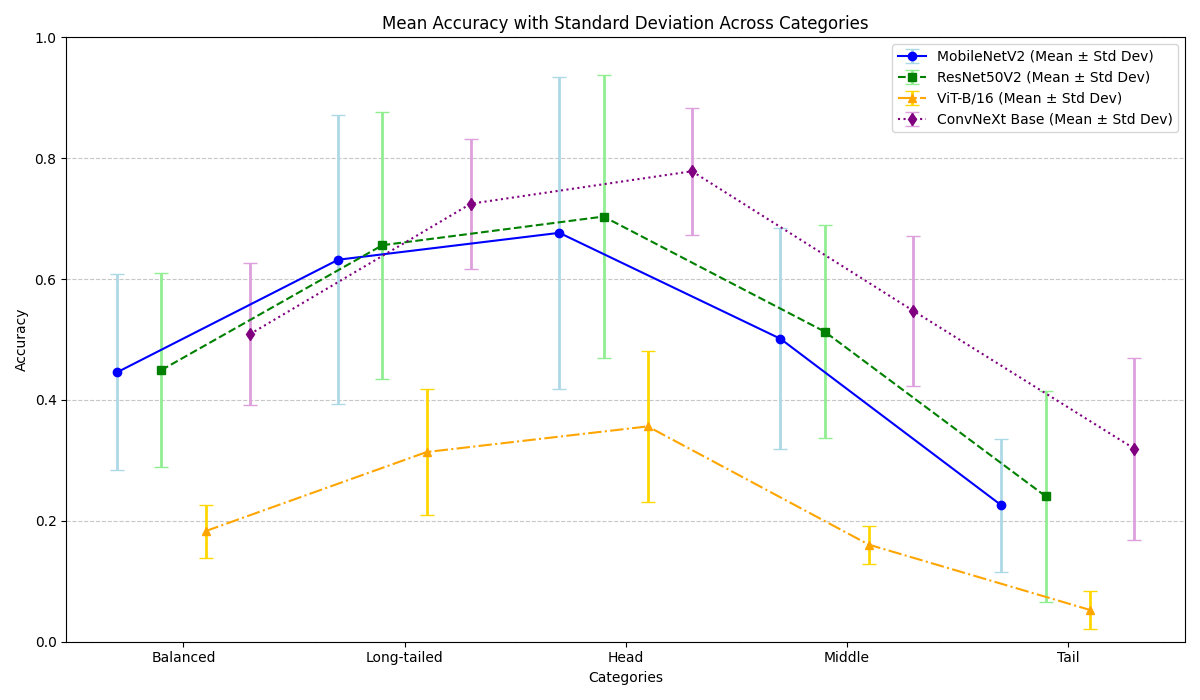
\includegraphics[width=\textwidth]{Images/Plots/mean_loss_comparison.png}
    \caption{Mean Accuracy with Standard Deviation Across Categories for MobileNetV2, ResNet50V2, ViT-B/16, and ConvNeXt Base.}
    \label{fig:mean_loss_comparison_line}
\end{figure}

\begin{figure}[h!]
    \centering
    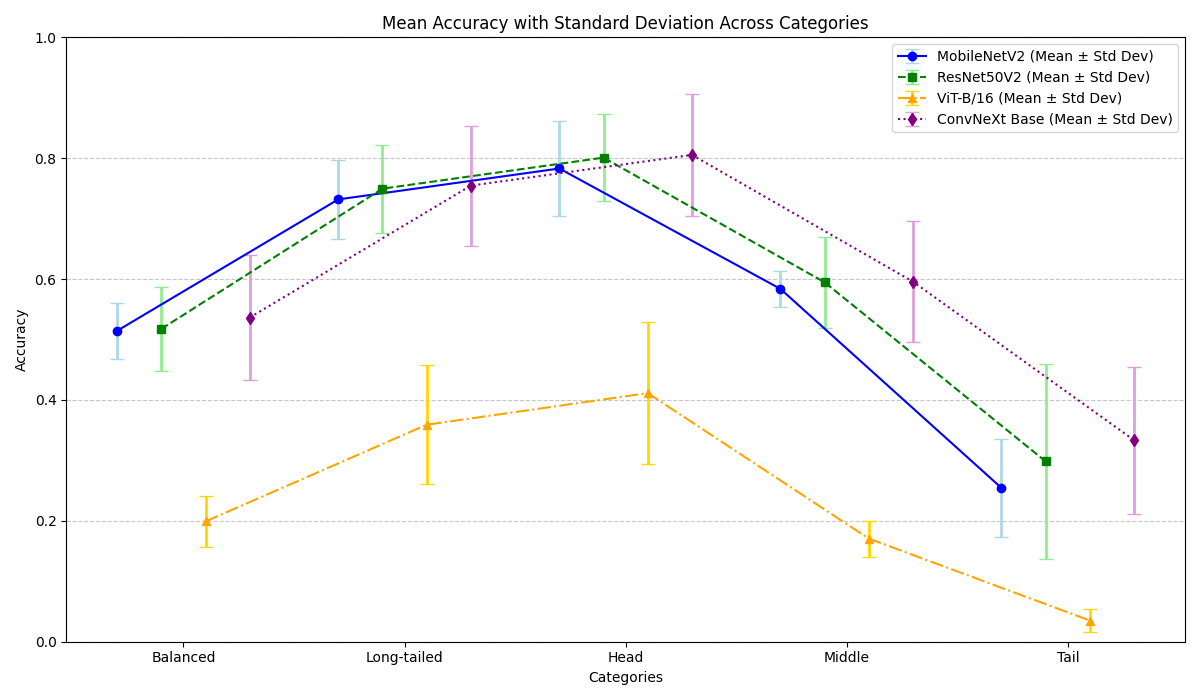
\includegraphics[width=\textwidth]{Images/Plots/mean_loss_comparison_noCB.png}
    \caption{Mean Accuracy with Standard Deviation Across Categories for MobileNetV2, ResNet50V2, ViT-B/16, and ConvNeXt Base without Class-Balanced Loss.}
    \label{fig:mean_loss_comparison_line_noCB}
\end{figure}


\todo{Comparison of overall model performance. Potentially statistical analysis, e.g. ANOVA, Tukey's HSD.}

\section{Comparison of Loss Functions}
\todo{Comment on the lack of results from the Class-Balanced Loss on all sets except the tail classes.} 

From figure \ref{fig:loss_comparison} it can be seen that the Balanced Softmax Loss has a better average perfomance on tail classes, while also displaying the smoothest variation across evaluation categories, ignoring the Class-Balanced loss. However, the standard deviation suggests that the perfomance of the Balanced Softmax Loss depend on the model architecture.

\begin{figure}[h!]
    \centering
    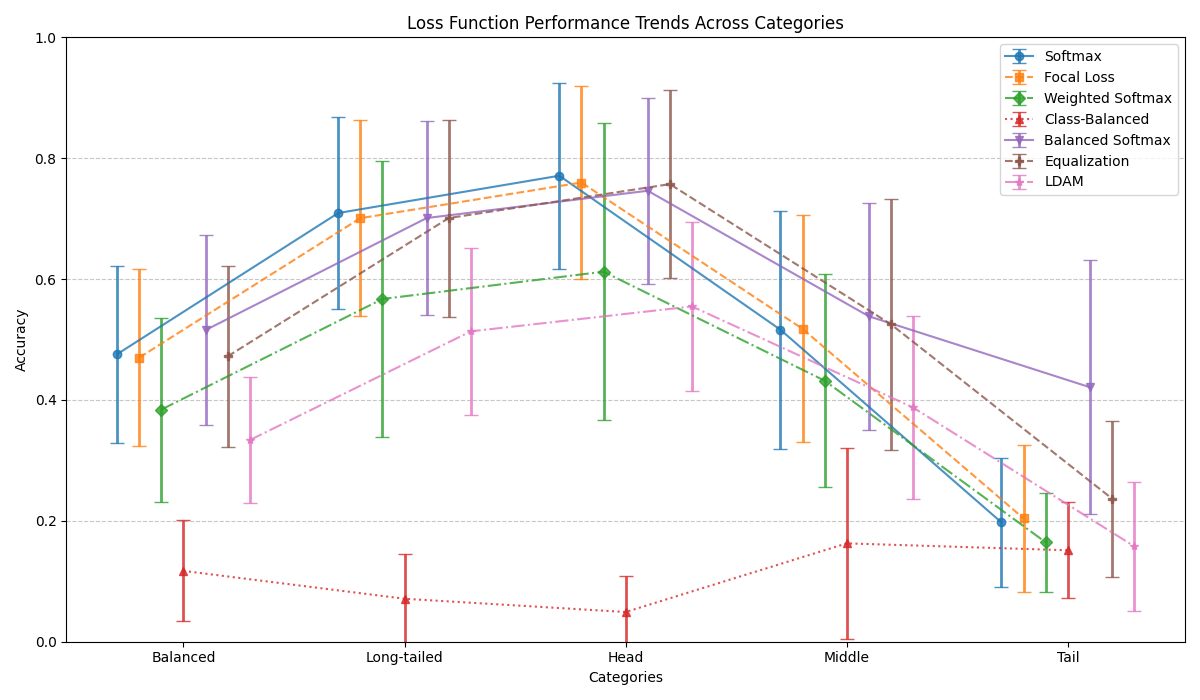
\includegraphics[width=\textwidth]{Images/Plots/loss_comparison.png}
    \caption{Performance trends of different loss functions across evaluation categories. Error bars indicate the standard deviation of accuracy across models, highlighting variability in performance for each loss function.}
    \label{fig:loss_comparison}
\end{figure}


\section{Comparison with Benchmarks}
The results are compared to the best published results for MobileNetV2, ResNet50V2, ViT-B/16 and ConvNeXt Base on CIFAR-100.

To contextualize the performance of models, the results are compared against the best posted results for the same architecture on CIFAR-100, reported by Author/Source.

\todo{Move benchmark results into a table.}

% Highlight Key Differences
% If there are differences in training conditions (e.g., data augmentation, optimization strategies, or hardware), acknowledge them:
% "It is important to note that while our setup involves an imbalanced CIFAR-100 dataset, the benchmark results were obtained on a balanced dataset."
% "Our experiments use an Adam optimizer, whereas [Source] employed SGD with momentum."

% \section{Qualitative Results}
% Include if time.
% Provide examples of correctly and incorrectly classified samples, especially for tail classes.
% Include visualizations or images of difficult cases to highlight challenges in tail-class prediction.

\section{Summary and Discussion}
Things for discussion:

\begin{itemize}
    \item Why is the performance on tail classes better than the performance on head and middle classes for the balanced training data, and what could it mean for the results on the long-tail training data?
    \item Running multiple of the same training to check for variance. What could this tell us in terms of statistical significance?
    \item The LDAM should be run with DRW as well. Compare to articles that run both LDAM and LDAM-DRW.
    \item Including or omitting the Class-Balanced Loss.
    \item Discuss why the ViT-B/16 model underperforms but shows excellent performance in other studies.
    \item Argue why the test data for CIFAR-100 was created from the training data instead of the validation data, and why or why not it would have been better to split the validation data instead.
\end{itemize}


The Balanced Softmax Loss proved to be the most effective loss function for tail classes, consistently achieving the highest accuracy on these classes across all models while also achieving competing results on other datasets. This results highlight its strenght in re-weighting logits to account for imbalanced datasets, particular for tail classes, where the Softmax baseline loss function falter. The synergy between Balanced Softmax and certain architectures, such as ConvNeXt Base, was espicially notable, suggesting that specific combinations of models and loss functions can achieve superior performance.

However, this improvement in tail-class accuracy often came with trade-offs. For example, while ResNet50V2 achieved a top 1 accuracy of 0.6053 on tail classes using Balanced Softmax, its head-class accuracy (0.8270) lagged behind ConvNeXt Base (0.8685). This trade-off highlights the challenge of optimizing for both head and tail classes simultaneously and indicates that Balanced Softmax prioritizes tail-class adjustments at the expense of head-class performance. \todo{mention statistical significance.}

Class-Balanced Loss, in contrast, consistently underperformed across all models and datasets. This discrepancy between its intended purpose and observed results suggests possible issues with its weighting strategy or implementation. Further investigation is necessary to understand these limitations and determine whether its performance can be improved.

Notably, the ViT-B/16 architecture underperformed significantly across all loss functions and datasets, with an the best accuracy of 59.06\% on a balanced training dataset compared to its benchmark of 93.95\%. This suggests that Vision Transformers, despite their reported success in other contexts, may require more data, longer training, or additional fine-tuning. The results indicate that the default ViT-B/16 architecture may not be well-suited for long-tailed datasets without further optimization.

While Balanced Softmax stood out as the most robust loss function overall, statistical validation is required to confirm the significance of these findings, particularly when comparing closely performing configurations. % For instance, the performance gap between Balanced Softmax and Softmax Loss on middle classes or long-tailed datasets could reflect inherent dataset characteristics rather than the superiority of the loss function alone.

Overall, these findings emphasize the importance of aligning loss functions with both dataset characteristics and model architectures to address the challenges of deep long-tailed learning. % They also highlight the need for a nuanced approach that balances improvements in tail-class accuracy with minimal trade-offs in head-class and overall performance.